\chapter{Results}
\section{Virtual Prototyping of Cell Signals}

During the course of this thesis, numerical simulations for the microchannel have been carried out. On the one side, a simulation about the shape of a \gls{gmr}-sensor signal of cells was performed, where the magnetic momentum was conveyed through \glspl{mnp} bound to their surface. On the other side, cell aggregates have been looked at in the same manner with different angles respective to the sensor. Both simulations were then correlated to a reference dipole, with the equivalent magnetic momentum distributed in the center of mass.\\
Additionally, the flow and shear field inside the channel was simulated numerically for the channel cross section as well as for a particle near the walls. A force equilibrium simulation was also established in a basic manner. \\
Every simulation was captured in a MATLAB class ``MRCyte'', which contains material parameters and constants for all simulations above.
\subsection{Numerical investigation of immunomagnetic label density and size on quantitative magnetoresistive sensing of single cells and cell aggregates}
In order to mimic a immunomagnetically labeled cell flowing over the sensor half bridge, the planar integral of the respective \acrfull{B} was solved analytically. Here, $\mathbf{r}_i$ specifies the distance vector of a single \gls{mnp} from the sensor plane. The magnetic flux density was converted by the \gls{gmr} to a resistive change $\mathbf{R}_{sig}$ by scaling it with the \gls{gmr}-sensitivity $S$ and subsequently into a signal voltage $\mathbf{V}_{sig}$ inside the bridge branch.(\cref{eq:magneticFluxIntegral, eq:GMR-signal, eq:voltage-signal})\\
In the numerical approach, \glspl{mnp} were randomly sampled on a sphere surface with an equivalent diameter of \SI{4}{\micro\meter} or \SI{8}{\micro\meter}. Then, the signal was computed for every \gls{mnp} during every timestep. Additionally, the \gls{mnp} distribution was rotated in every iteration to resemble a rolling motion. The computed signals were then cross-correlated to the signal of a reference flux density $\mathbf{B}_{ref}$ caused by a point-like magnetic moment located in the geometric center of the same sphere.
\begin{align}
	\mathbf{B}(t) &= \sum_{i=1}^{N} \frac{1}{A_{\mathrm{Sensor}}} \int_{-\frac{l}{2}}^{\frac{l}{2}} \int_{-\frac{w}{2}}^{\frac{w}{2}} \frac{\mu_{o}}{4 \pi}\left(\frac{3 \mathbf{r}_{i}(t)\left(\mathbf{r}_{i}(t) * \mathbf{m}_{i}\right)}{\left|\mathbf{r}_{i}(t)\right|^{5}}-\frac{\mathbf{m}_{i}}{\left|\mathbf{r}_{i}(t)\right|^{3}}\right) dx dy \label{eq:magneticFluxIntegral} \\
	\mathbf{R}_{sig}(t) &= - \mathbf{B}(t) * \frac{S}{100} * R + R \label{eq:GMR-signal}\\
	\mathbf{V}_{sig}(t) &= \frac{\mathbf{R}_{sig}(t)}{R + \mathbf{R}_{sig}(t)}*V_p - \frac{V_p}{2} \label{eq:voltage-signal}
\end{align}
By its formula, cross-correlation $R_{x y}(\tau)$ yields a displacement dependent signal through its convolution of the complex conjugated reference signal $\mathrm{V}_{ref}^{*}(t)$ with the sample signal $\mathbf{V}_{sig}(t+\tau)$.(\cref{eq:xcorr}) Therefor, only the maximal correlation of this function was considered in further analyses.
\begin{equation}
	\mathrm{max}\{R_{x y}(\tau)\}=\mathrm{max}\left\{\int_{-\infty}^{\infty} \mathrm{V}_{ref}^{*}(t) \mathbf{V}_{sig}(t+\tau) dt \right\} \label{eq:xcorr}
\end{equation}
\todo{Signal Similarity For Cells With Varying Bead Coverages,Cross-Correlation between single dipole with sum magentic moment and surface covered with randomly distributed magnetic particles, simulation of cell rolling velocity and forces}

%\\nas.ads.mwn.de\tuze\t03\AG-Hayden Studenten\00_Students\Johann Brenner\02_software\01-MRCyte\Magnetic cytometry signal modeling
\subsection{Single Cell Signal}
Aim of these simulations is to find a measure of how magnetic labelling of a cell affects signal shape and its subsequent analysis. A single cell with a surface coverage of \SIrange{5}{99}{\percent} of a densely packed sphere was loaded randomly with \glspl{mnp} at different sizes. As shown in the schematic \cref{fig:sim:intro:coverage}, not only signal peak amplitude but also \gls{fwhm} increases at growing coverages. 

\begin{figure}[htb]
	\centering
	\subfloat{
		\subfigimg[height=80pt]{a}{Ressources/Simulation/ParticleCoverage}
		\phantomsubcaption
		\label{fig:sim:intro:coverage}
		} \hfill
	\subfloat{
		\subfigimg[height=80pt]{b}{Ressources/Simulation/ParticleAngle}			
		\phantomsubcaption
		\label{fig:sim:intro:angle}
	} 
	\subfloat{
	\subfigimg[height=80pt]{c}{Ressources/Simulation/GMR}			
	\phantomsubcaption
	\label{fig:sim:intro:gmr}
} 
	\capption{Particle Coverage Simulation}{(\textbf{a}) The single ideal magnetic dipole in the center  (\blueCircle) causes a signal deviation from the real cell signal with magnetic moment distributed on the cell surface (\orangeCircle) (\textbf{b}) Signal shapes of different angles of 2-particle aggregates (\textbf{c}) GMR Sensor simulation dimensions}
	\label{fig:sim:intro}	
\end{figure}

%Überlegen, ob grafik in einen große 

simulation Parameters


why the cell signal differs --> number of aggregates --> single particle moments are more weighted

PArticle size is dependent --> number less, but moment higher --> single particle is even more important

\begin{figure}
	\centering
	\subfloat{	
		\subfigimg[height=145pt]{b}{Ressources/Simulation/Small2um}	
		\phantomsubcaption
		\label{fig:sim:coverage:small2um}
	} \hfill
	\subfloat{
		\subfigimg[height=145pt]{a}{Ressources/Simulation/Big2um}
		\phantomsubcaption
		\label{fig:sim:coverage:big2um}	
	} \\
	\vspace{\baselineskip}
	\subfloat{	
		\subfigimg[height=145pt]{d}{Ressources/Simulation/Small4um}	
		\phantomsubcaption
		\label{fig:sim:coverage:small4um}
	}\hfill
	\subfloat{
		\subfigimg[height=145pt]{c}{Ressources/Simulation/Big4um}
		\phantomsubcaption
		\label{fig:sim:coverage:big4um}
	}
\capption{Coverage Dependent Signal Correlation}{Mean from 3 differently distributed particles, SEM (\textbf{a}) d = \SI{4}{\micro\meter} (\textbf{b}) d = \SI{4}{\micro\meter} (\textbf{c}) d = \SI{8}{\micro\meter} (\textbf{d}) d = \SI{8}{\micro\meter}}
\label{fig:sim:coverage}
\end{figure}



\begin{figure}
		\centering
	\subfloat{
		\subfigimg[height=150pt]{a}{Ressources/Simulation/CorrelationDiff2um}	
	} \hfill
	\subfloat{
		\subfigimg[height=150pt]{b}{Ressources/Simulation/CorrelationDiff4um}	
	}
\capption{Difference of Cross-Correlation at Maximum Coverage}{Mean from 3 different particle distributions at maximum coverage(\textbf{a}) d = \SI{4}{\micro\meter} (\textbf{b}) d = \SI{8}{\micro\meter}}
\label{fig:sim:CorrDiff}
\end{figure}

\subsection{Cell Aggregates}

\begin{figure}	
	\centering
	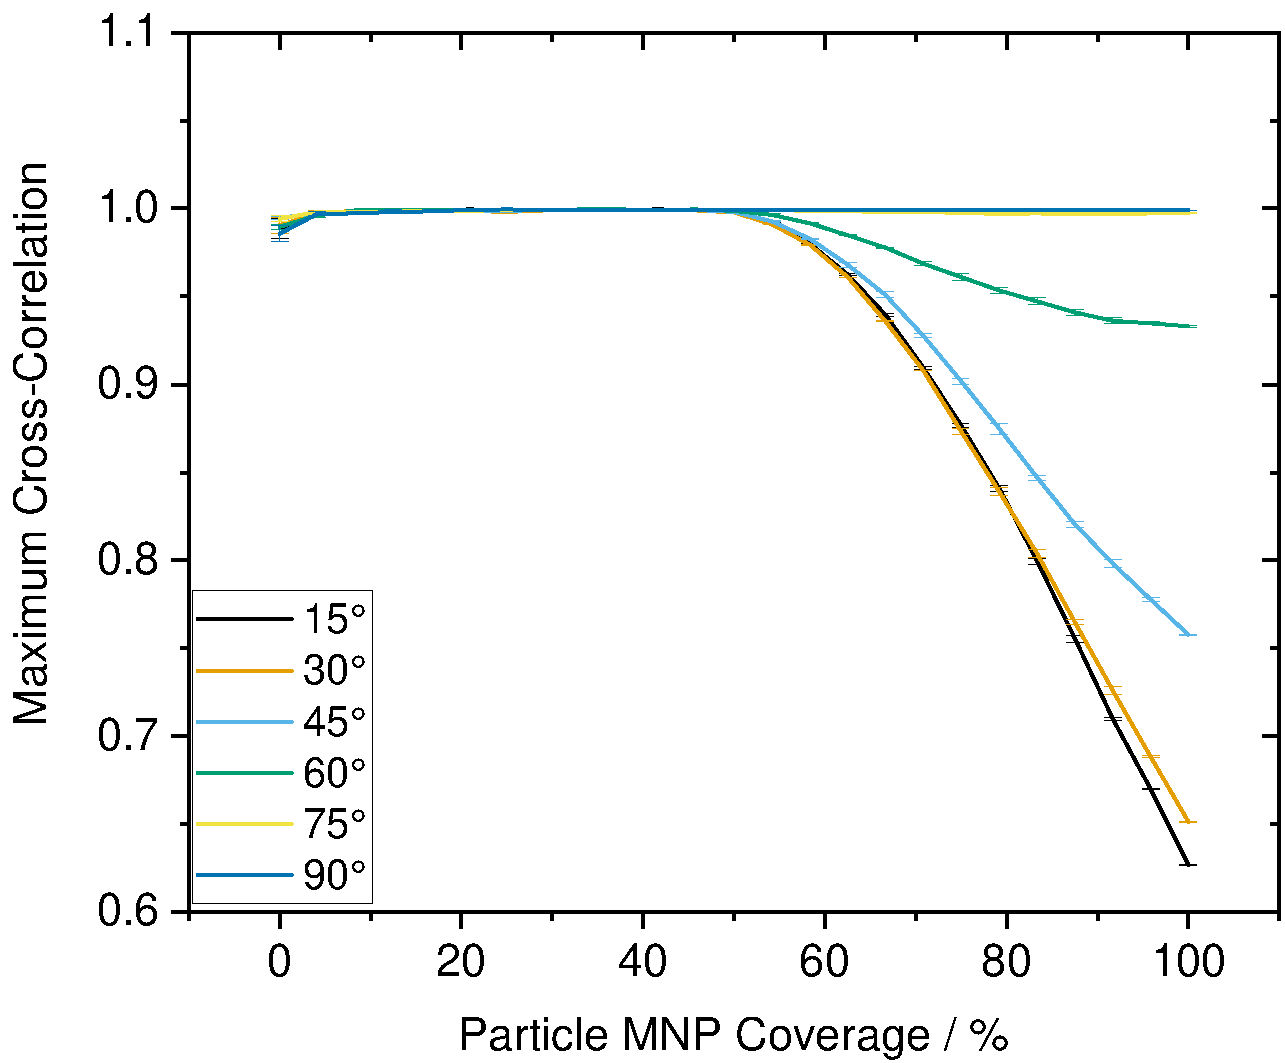
\includegraphics[width=.7\linewidth]{Ressources/Simulation/Aggregates}	
	\capption{Sensor Signals Correlation between Two Cell Aggregates At Shifting Angles with a Reference Dipole}{Mean from 3 differently distributed particles, SEM}
	\label{fig:sim:aggregates}
\end{figure}

\section{Reference Bead Surface Functionalization}



\subsection{Amine-Surface Biotinylation}
Streptavidin-Atto488 reference calibration
Anti-Biotin-PE working?
BNF-Dextran-Streptavidin unspecific binding?



\begin{figure}[htb!]
	\centering
	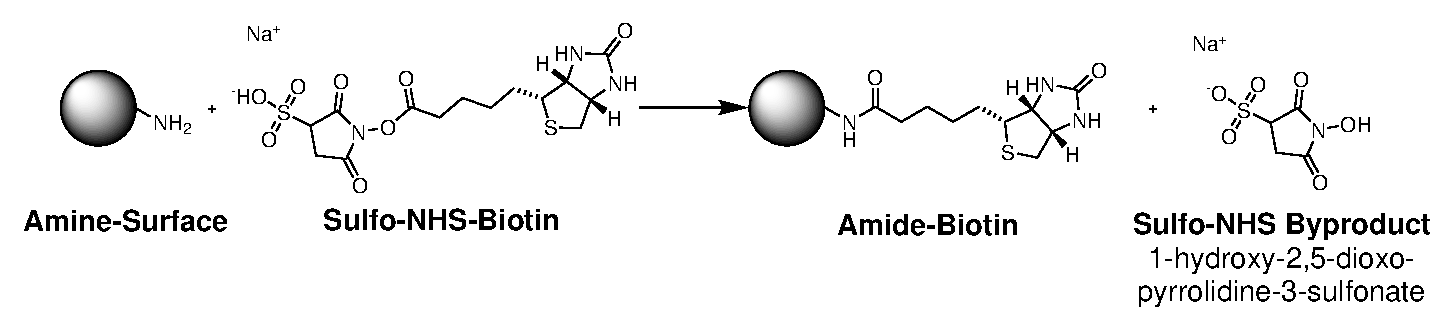
\includegraphics[width=\linewidth]{./Ressources/Chemistry/Sulfo-NHS.eps}
	\capption{Amine Bead Modification with Sulfo-NHS-Biotin}{An amine terminated bead is incubated with sulfo-NHS-Biotin to cover its surface by amide-Biotin. As byproduct the sulfo-NHS-ester 1-hydroxy-2,5-dioxopyrrolidine-3-sulfonate splits off. }
	\label{fig:Chem:NH2-NHS}
\end{figure}


\begin{figure}[htb!]
	\centering
	\subfloat{
		\subfigimg[height=90pt]{a}{./Ressources/Biotinyl/mag-nh2}	
	} \hfill
	\subfloat{
		\subfigimg[height=90pt]{b}{./Ressources/Biotinyl/cooh}	
	}\hfill
	\subfloat{
		\subfigimg[height=90pt]{c}{./Ressources/Biotinyl/IgG-cooh}	
	} \\
\vspace{\baselineskip}
	\subfloat{
	\subfigimg[height=150pt]{c}{./Ressources/Biotinyl/stability}	
	}

	\capption{Titration of Biofunctional Molecules on \SI{8}{\micro\meter} Particles}{ (\textbf{a}) NHS-Biotin, MFI, CV, reduced chi square = 275.19597, Hill Fit $y=Vmax*x^n/(k^n+x^n)$, Vmax = 173.077, k = 0.0572831, n = 1.63554 (\textbf{b}) Amin-PEG$_2$-Biotin MFI, CV, outlier neglected Gleichung: $y=Vmax*x^n/(k^n+x^n)$ Vmax	171,02602, k   	0,04201, n   	0,91338,Chi-Quadr Reduziert	4,07387	(\textbf{c}) MFI, CV, reduced chi square = 0.91011, Hill Fit $y=Vmax*x^n/(k^n+x^n)$, Vmax = 713.83643, k = 182.83011	, n = 0.72458  (\textbf{d}) MFI, SEM, $\tau_{decay}$ = \num{1.42557 +- 0.16188}	Equation	$y = A \exp^\frac{-x}{\tau_{decay}} + y_0$	y0	0.12369 ± 0.01576	A1	0.91263 ± 0.06964	t1	1.42557 ± 0.16188	Reduced Chi-Sqr	0.00542 }
	\label{fig:biotinyl:titration}
\end{figure}



%\begin{figure}[htb!]
%	\centering
%	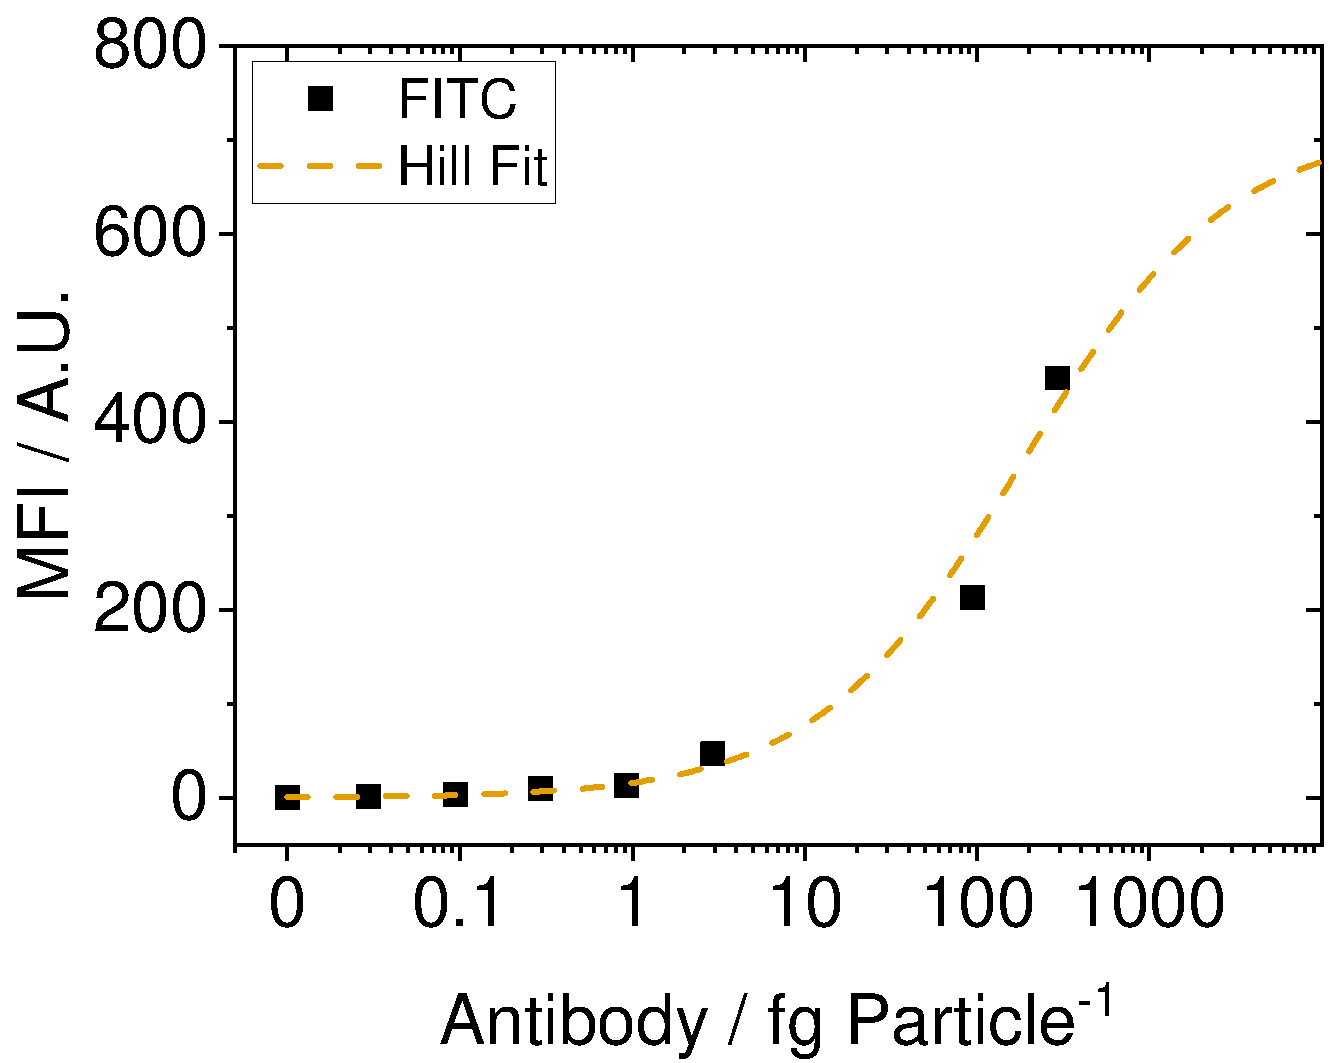
\includegraphics[width=.7\linewidth]{./Ressources/Biotinyl/IgG-cooh}
%	\capption{Titration of Anti-IgG1 on \SI{8}{\micro\meter} Particles}{MFI, CV, reduced chi square = 
%		0.91011, Hill Fit $y=Vmax*x^n/(k^n+x^n)$, Vmax = 713.83643, k = 182.83011	, n = 0.72458 }
%	\label{fig:biotinyl:IgG-cooh}
%\end{figure}

%\begin{figure}[htb!]
%	\centering
%	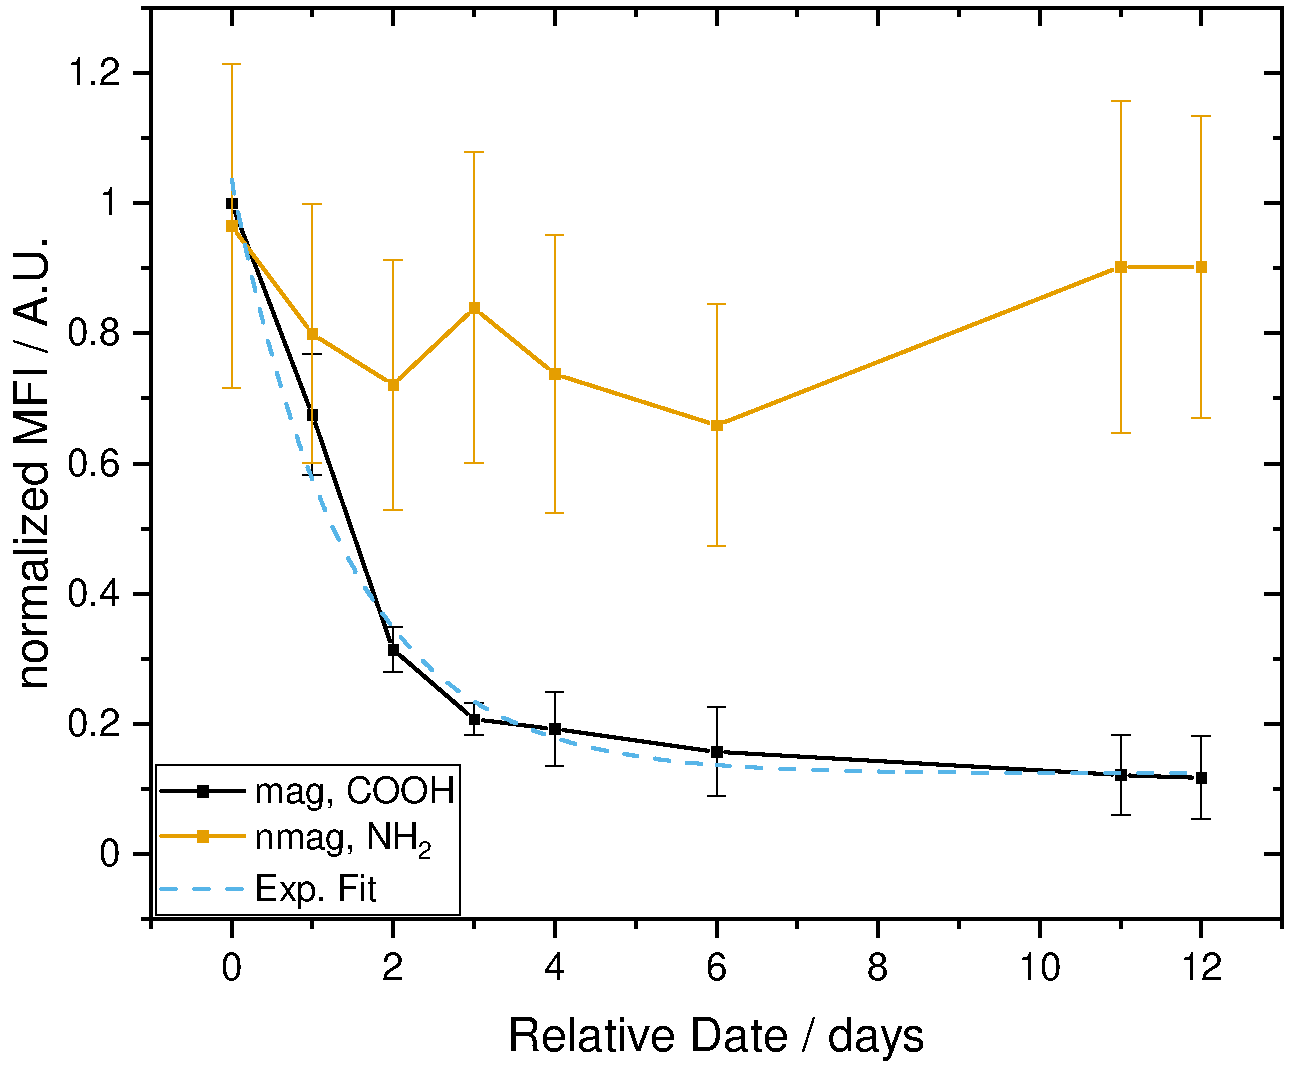
\includegraphics[width=\.7\linewidth]{./Ressources/Biotinyl/stability}
%	\capption{Titration of Anti-IgG1 on \SI{8}{\micro\meter} Particles}{MFI, SEM, reduced chi square = 
%		0.00542, Hill Fit $y=Vmax*x^n/(k^n+x^n)$, Vmax = 713.83643, k = 182.83011	, n = 0.72458 }
%	\label{fig:biotinyl:stability}
%\end{figure}


\section{Concentration Measurements in MRCyte}
Explain v-c
\begin{figure}[htb!]
	\centering
	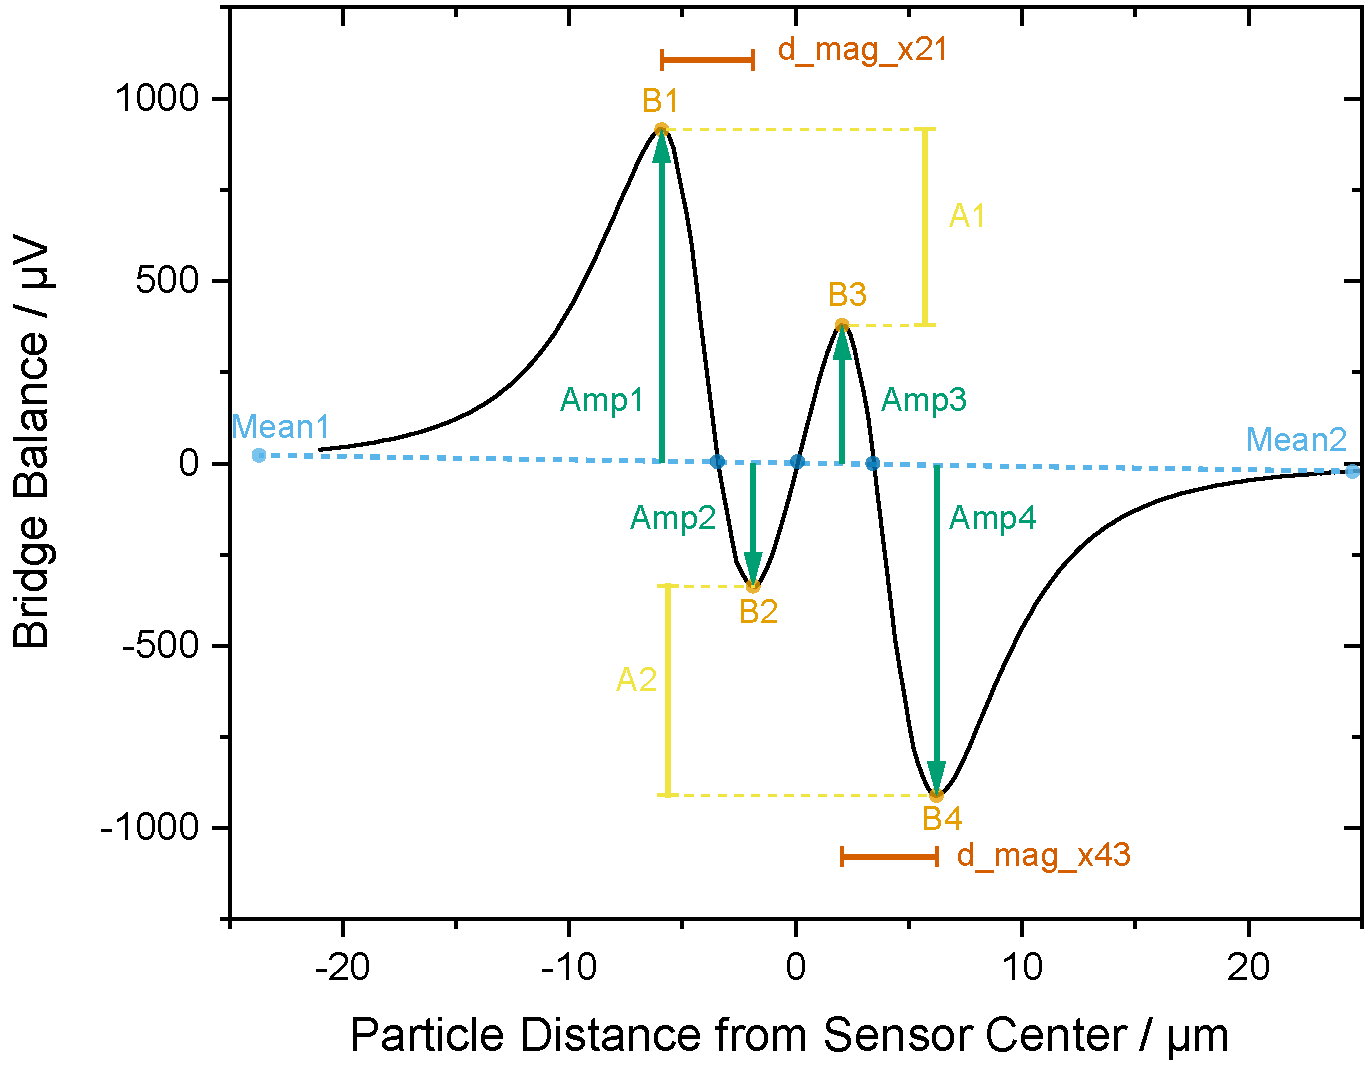
\includegraphics[width=.7\linewidth]{Ressources/Simulation/ExampleSignal}
	\capption{Example Signal of Magnetic Measurement}{explain all}
	\label{fig:conc:example}
\end{figure}

\begin{figure}[htb!]
	\centering
	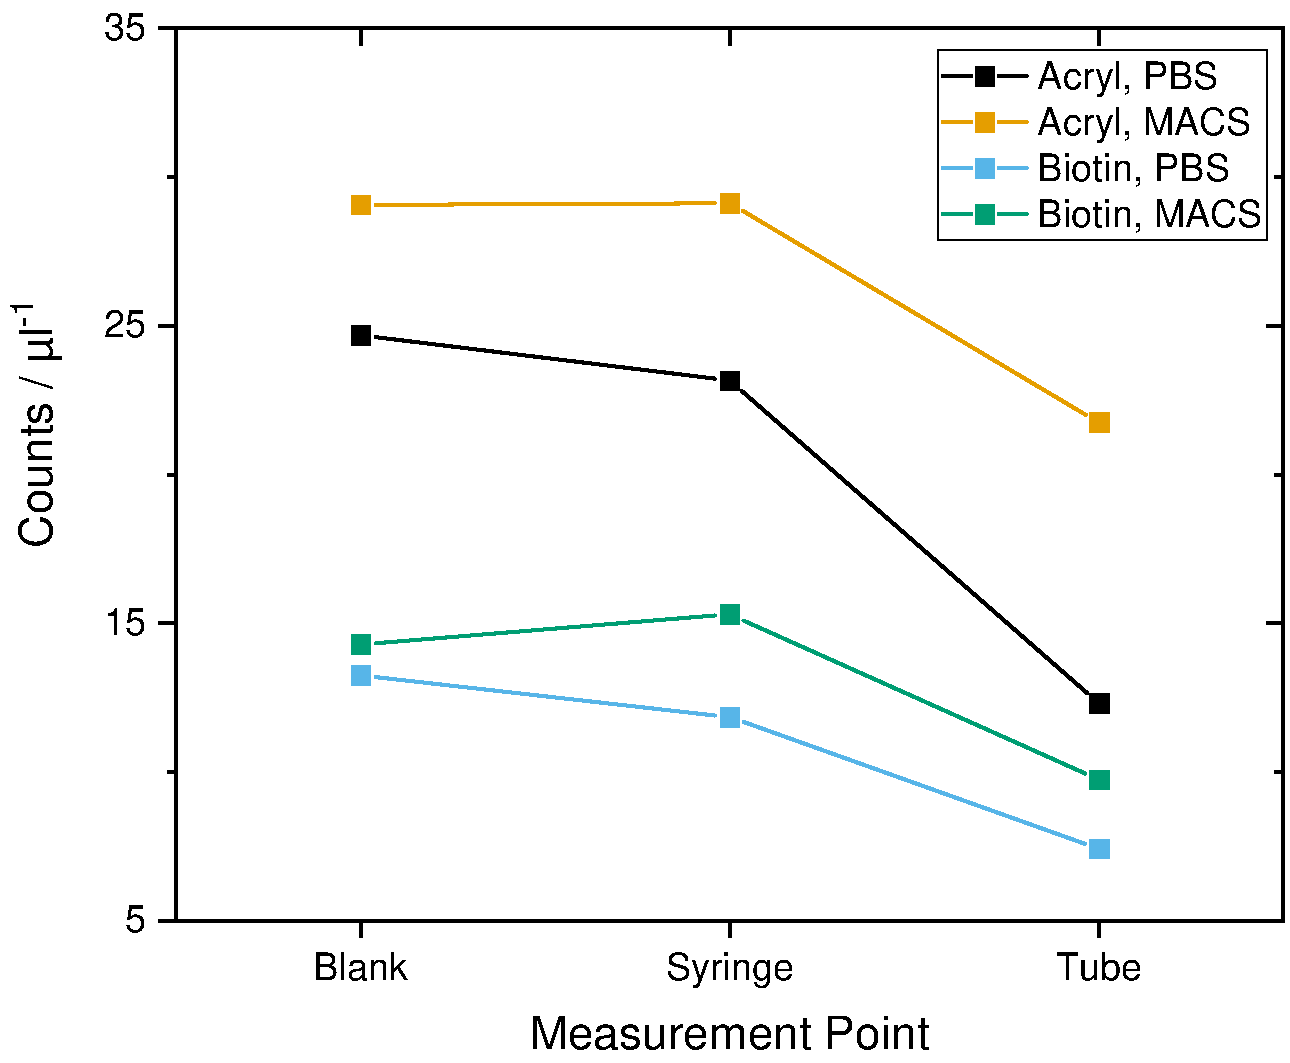
\includegraphics[width=.7\linewidth]{Ressources/Concentration/Losses-Syringe-Tubing}
	\capption{Bead Loss Evaluation in Connectors}{Losses in different buffers and bead surfaces.}
	\label{fig:conc:losses_syringe}
\end{figure}



\subsection{Calibration of Flow Field}
\begin{figure}
	\centering
	\subfloat{
		\subfigimg[height=150pt]{a}{Ressources/Concentration/ConcentrationError}	
	} \hfill
	\subfloat{
		\subfigimg[height=150pt]{b}{Ressources/Concentration/ConcentrationVelocity}	
	}
	\capption{Absolute Concentration Measurements}{Mean from 3 independent measurements(\textbf{a}) mean, sd (\textbf{b}) mean, SEM, Reference Count based error: Liner fit steepness \num{0,34622 +- 0,00968} --> Correction Factor (inverse) \num{2,88833 +- 0,08075}, Velocity Based Correction: $Q/A$ Dims: \SI{700}{\micro\meter}x\SI{50}{\micro\meter} Q = \SI{30}{\micro\liter\per\minute} --> \num{2,26109}}
	\label{fig:conc:AbsConcError}
\end{figure}

\begin{figure}
	\centering
	\subfloat{
		\subfigimg[height=150pt]{a}{Ressources/Concentration/BiotinylWrongCorrection}	
	} \hfill
	\subfloat{
		\subfigimg[height=150pt]{b}{Ressources/Concentration/BiotinylTime}	
	}
	\capption{Error Sources in Concentration Measurements}{(\textbf{a}) mean, SEM Fit factor comparison with protein coated surfaces (\textbf{b}) mean, SEM}
	\label{fig:conc:BiotnylWrongCorr}
\end{figure}

\subsection{Count Stability}
Measurement over 1h

\begin{figure}[!h]
	\centering
	\subfloat{
		\subfigimg[height=150pt]{a}{Ressources/Concentration/BiotinylCountAll}	
	} \hfill
	\subfloat{
		\subfigimg[height=150pt]{b}{Ressources/Concentration/BiotinylTimeAll}	
	}
	\capption{Reproducibility of Concentration Measurements with Saturated Neutravidin Surface}{(\textbf{a}) \SI{80}{\micro\liter\per\minute} mean, SEM (\textbf{b}) All,mean, SEM,}
	\label{fig:conc:All}
\end{figure}



\begin{figure}[htb!]
	\centering
	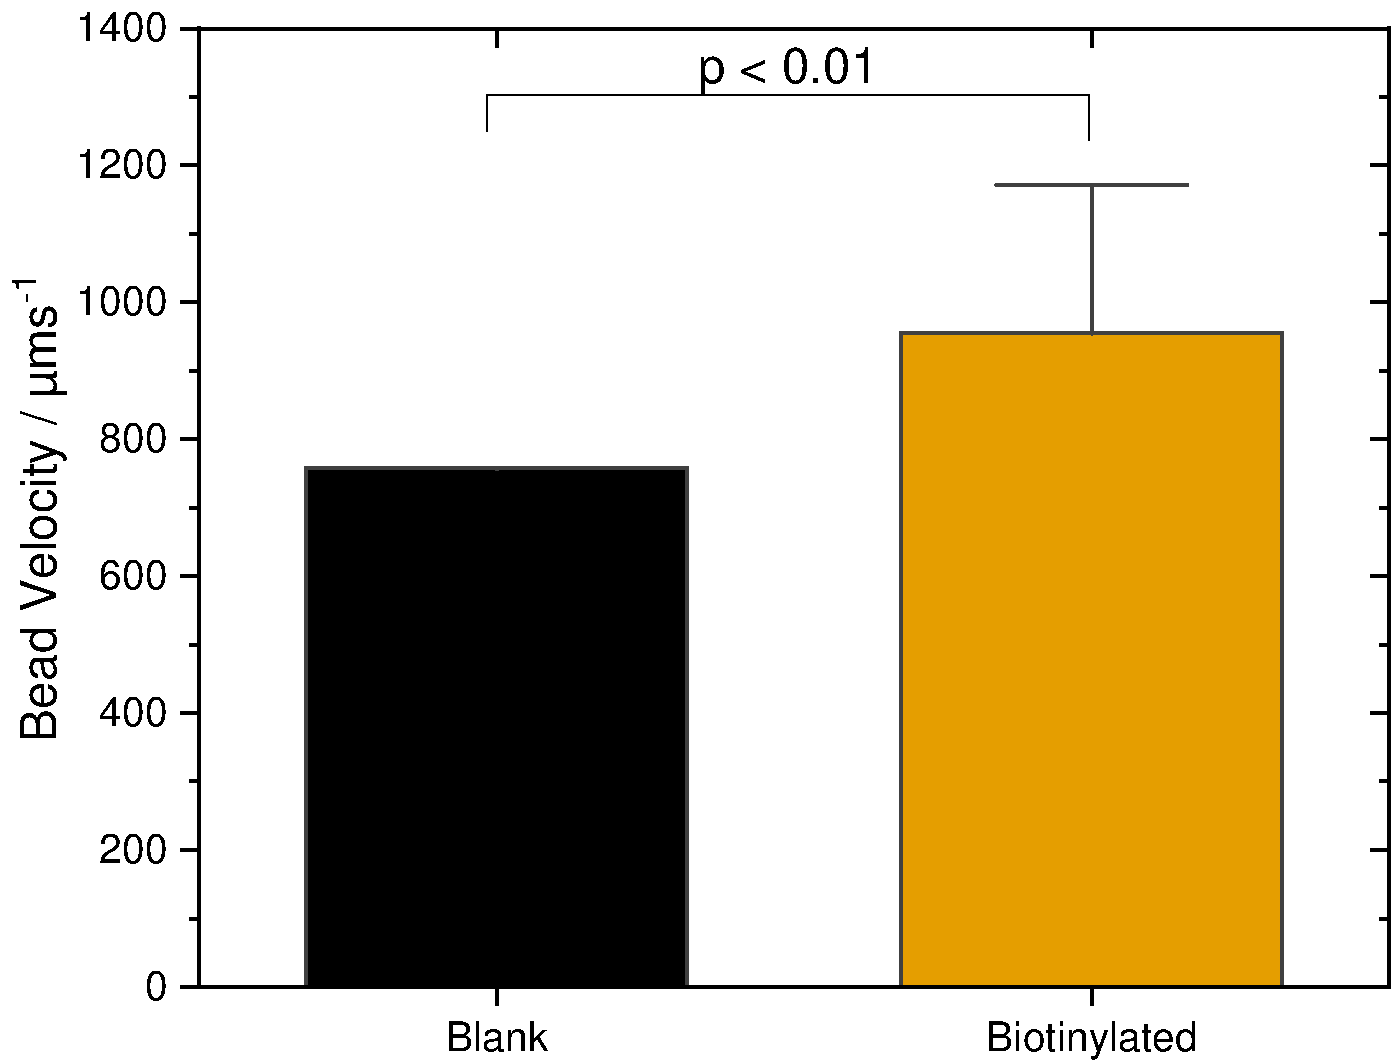
\includegraphics[width=.7\linewidth]{Ressources/Concentration/CaptureVelocity}
	\capption{Measured Bead Velocity}{ p < 0.01}
	\label{fig:conc:vel}
\end{figure}




\subsubsection{Concentration Measurement in Diluted Whole Blood}


\begin{figure}[htb!]
	\centering
	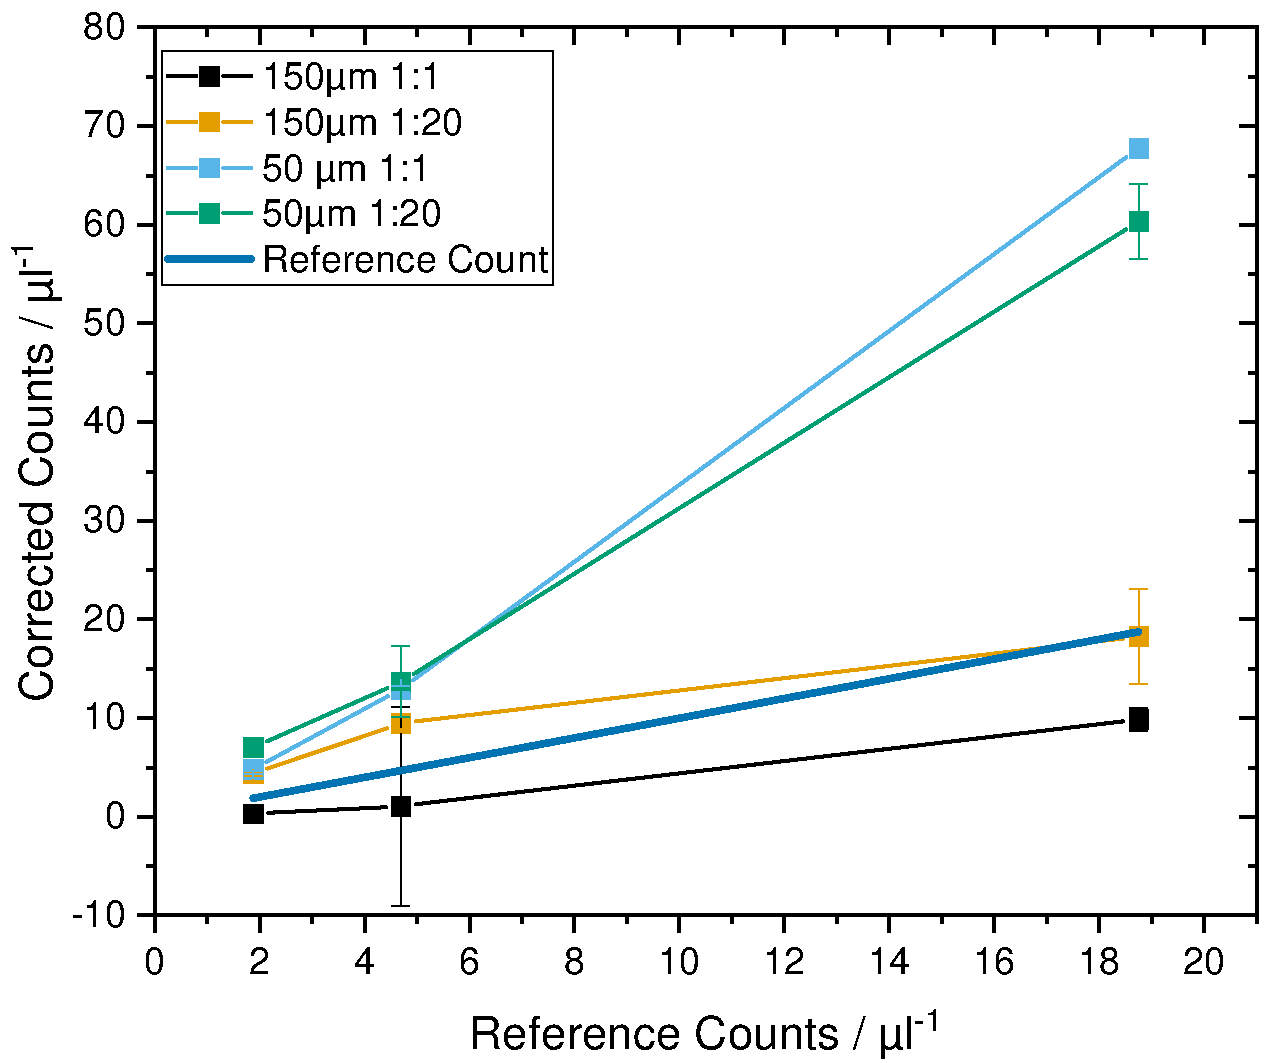
\includegraphics[width=.7\linewidth]{Ressources/Concentration/CorrectionBlood}
	\capption{Absolute Concentration Measurement in Blood Samples Under Varying Channel Height}{Velocity Correction does not work for high concentrations in \SI{50}{\micro\meter}}
	\label{fig:conc:blood}
\end{figure}




\subsection{Differential Counting Setup}

\subsubsection{Sensitivity Calibration}

\begin{figure}[!h]
	\centering
	\subfloat{
		\subfigimg[height=150pt]{a}{Ressources/Differential/Optupper}	
	} \hfill
	\subfloat{
		\subfigimg[height=150pt]{b}{Ressources/Differential/Optlower}	
	}
	\capption{Hysteresis Calibration for Stacked \Gls{pcb} }{(\textbf{a}) Optimized for top sensor (\textbf{b}) Optimized for bottom sensor}
	\label{fig:diff:sensitivity}
\end{figure}

\subsubsection{Concentration Measurement in Buffer Solution}



\begin{figure}[!h]
	\centering
	\subfloat{
		\subfigimg[height=150pt]{a}{Ressources/Differential/Bottom}	
	} \hfill
	\subfloat{
		\subfigimg[height=150pt]{b}{Ressources/Differential/Top}	
	}
	\capption{Flow Rate Dependency of Counting Setup}{(\textbf{a}) Optimized for top sensor (\textbf{b}) Optimized for bottom sensor}
	\label{fig:diff:flowRate}
\end{figure}

\begin{figure}[htb!]
	\centering
	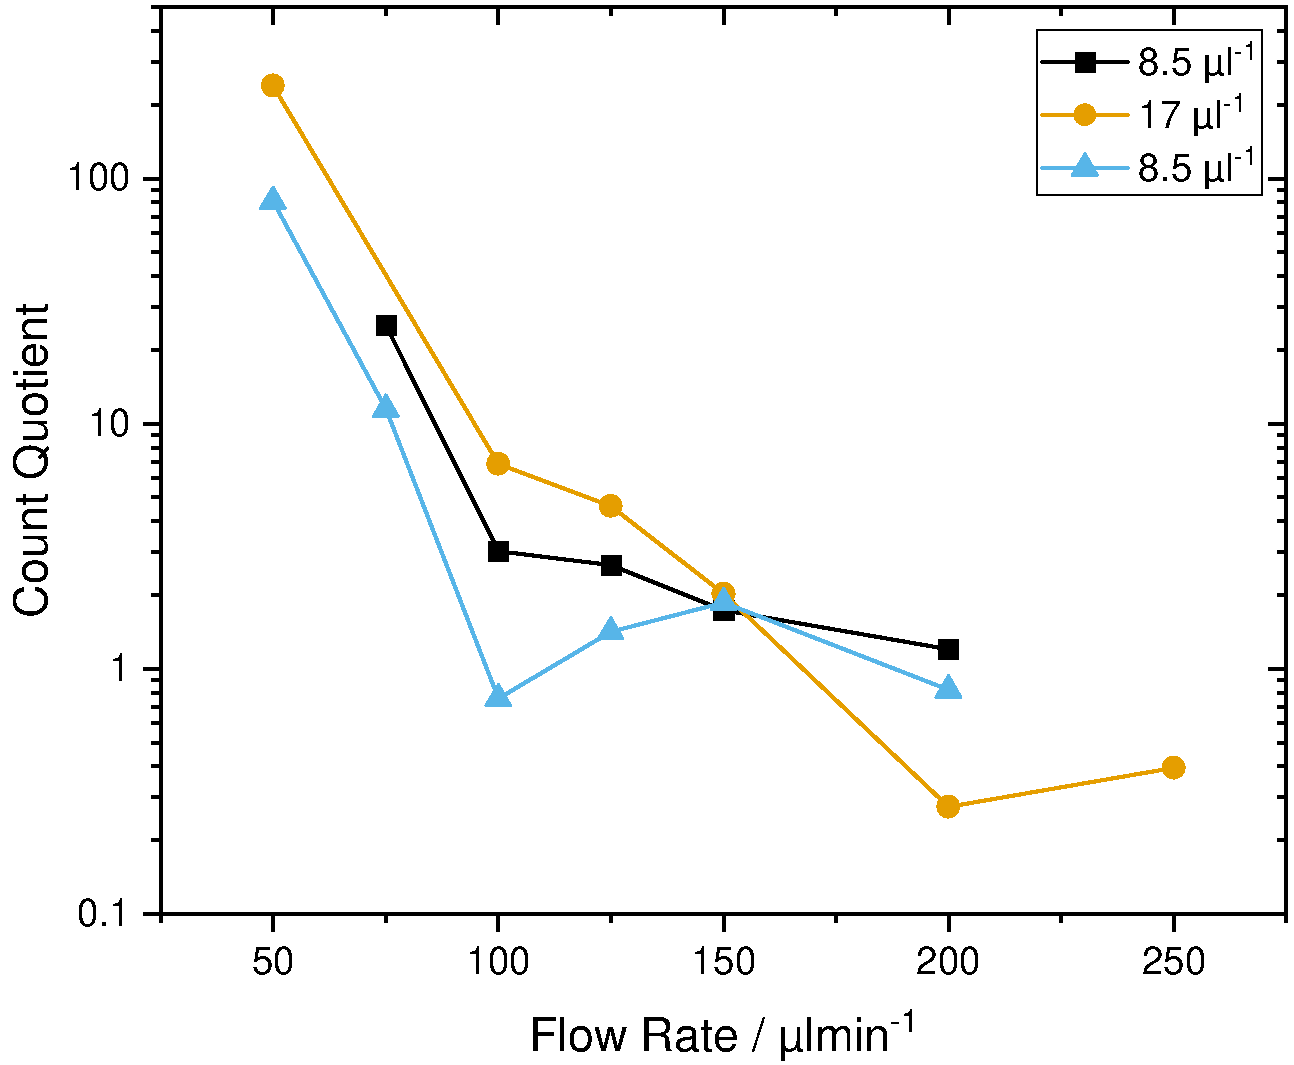
\includegraphics[width=.7\linewidth]{Ressources/Differential/Differential}
	\capption{Optimal Differential Counting Flow Rate}{Losses in different buffers and bead surfaces.}
	\label{fig:conc:optimum}
\end{figure}




\subsection{Surface Magnetization of Biofunctionalized Beads}

Somehow BNF-Dextran showed unspeficity initally, but not anymore later on

\begin{figure}[!h]
	\centering
	\subfloat{
		\subfigimg[height=150pt]{a}{Ressources/Concentration/BNFC1}	
	} \hfill
	\subfloat{
		\subfigimg[height=150pt]{b}{Ressources/Concentration/BNFVc}	
	}
	\capption{Bead Coverage Assay with BNF-Dextran-redF-\SI{100}{\nano\meter}}{(\textbf{a}) 1. \SI{80}{\micro\liter\per\minute} 2. \SI{40}{\micro\liter\per\minute} 3. \SI{20}{\micro\liter\per\minute} 4. \SI{10}{\micro\liter\per\minute} (\textbf{b}) d = \SI{8}{\micro\meter}}
	\label{fig:conc:BNF}
\end{figure}



\begin{figure}[!h]
\centering
\subfloat{
	\subfigimg[height=150pt]{a}{Ressources/Concentration/OceanC1}	
} \hfill
\subfloat{
	\subfigimg[height=150pt]{b}{Ressources/Concentration/OceanVc}	
}
\capption{Bead Coverage Assay with OceanNanotec \SI{50}{\nano\meter}}{Mean from 3 different particle distributions at maximum coverage, SEM(\textbf{a}) d = \SI{4}{\micro\meter} (\textbf{b}) d = \SI{8}{\micro\meter}}
\label{fig:conc:Ocean}
\end{figure}


\section{Surface Modification and Biofunctionalization of the Sensor Chip Substrate}

\subsection{Physisorption}
Quantification in Plate Reader
Trial with Neutravidin + Sensor (Esthis Versuch)
\clearpage

\begin{figure}
	\centering
	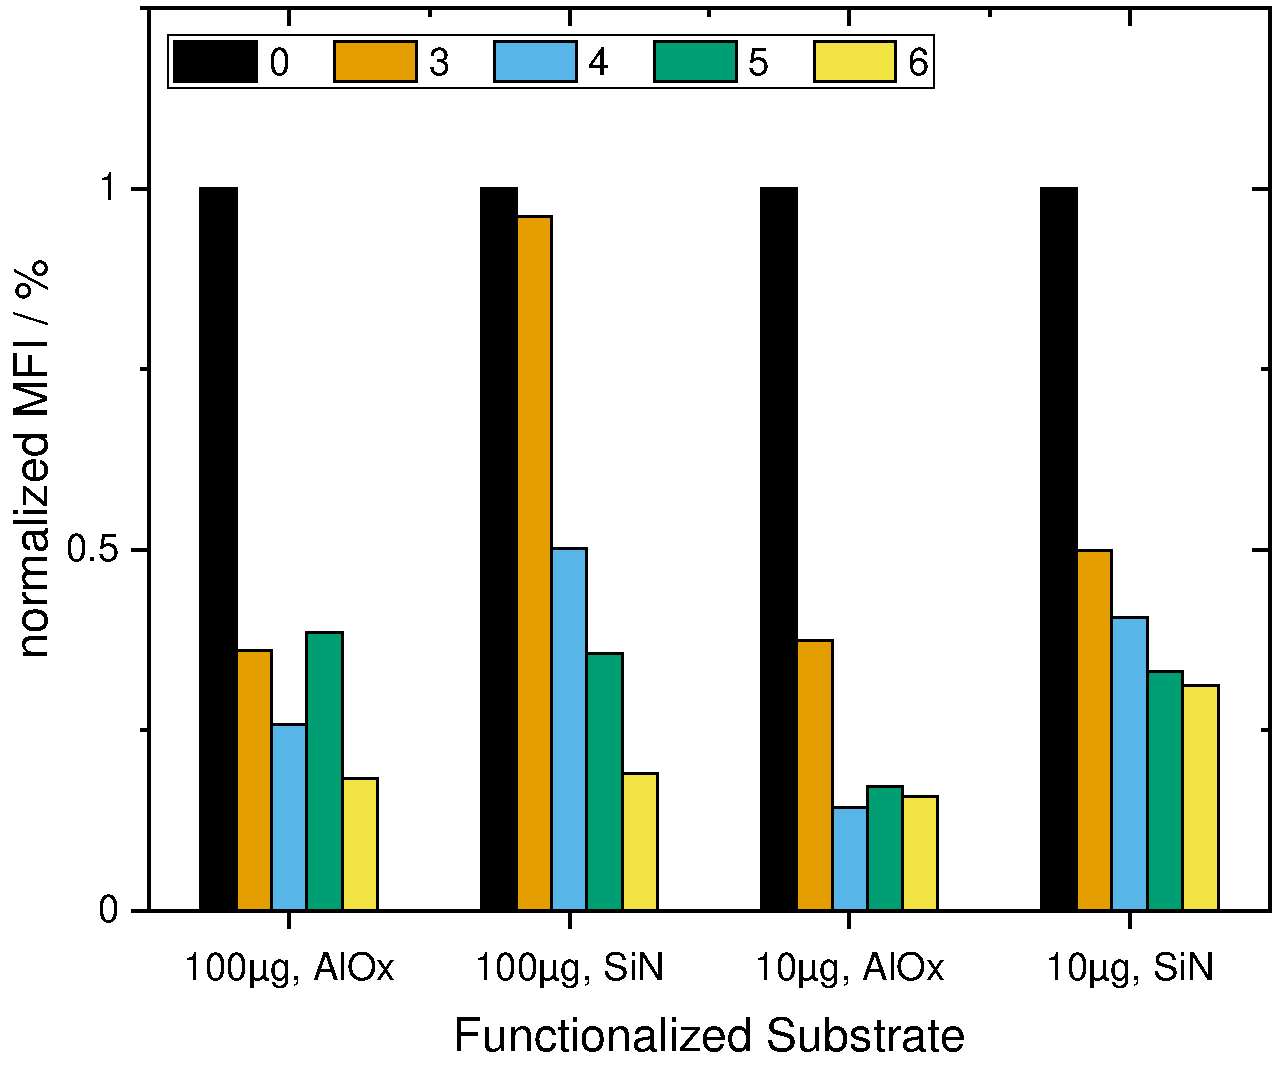
\includegraphics[height=150pt]{Ressources/ResultPlots/SurfaceFuncSiNAlOx}
	\capption{Surface Adsorption Stability of Neutravidin on \Gls{sin} and \Gls{alox}}{Blank with PBS and Blank substrate, corrected, then normalized, absolute protein per \textasciitilde \SI{25}{\milli\meter\square}}
	\label{fig:unsp:wash}
\end{figure}


\subsection{Covalent Attachment}
%\clearpage


\begin{figure}[htb!]
	\centering
	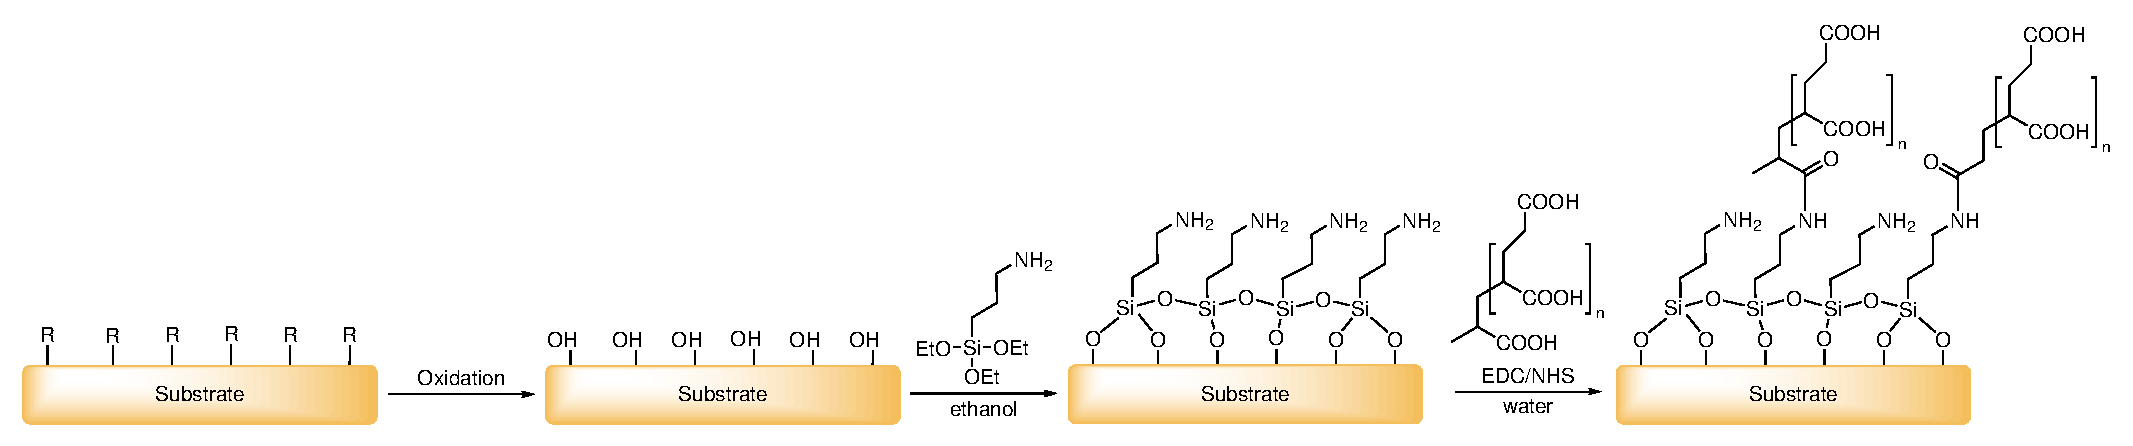
\includegraphics[width=1\linewidth]{Ressources/Chemistry/Substrate}
	\capption{General process chain of chemical surface modification}{Any substrate with various surface groups R (\textbf{a}) is oxidized to exhibit \gls{hydroxyl} groups.(\textbf{b}). Then a silane \gls{sam} is attached (\textbf{c}) and subsequently modified by carbodiimide chemistry with \gls{paa}. (\textbf{d})}
	\label{fig:chem:func:withPAA}
\end{figure}


\begin{figure}[!h]
	\centering
	\subfloat{
		\subfigimg[height=150pt]{a}{Ressources/Covalent/SerpentinesDensityCount}	
	} \hfill
	\subfloat{
		\subfigimg[height=150pt]{b}{Ressources/Covalent/NeutravidinTitration}	
	}
	\capption{Neutravidin Titration Fluorescence and Bead Capture Assay}{Relate count to area, then change MFI to counts \si{\per\micro\liter\per\milli\meter\squared}(\textbf{a}) Serpentine (\textbf{b}) Glass}
	\label{fig:coval:fluo}
\end{figure}

\subsubsection{Plasma-Based Approach}
\begin{figure}
	\centering
	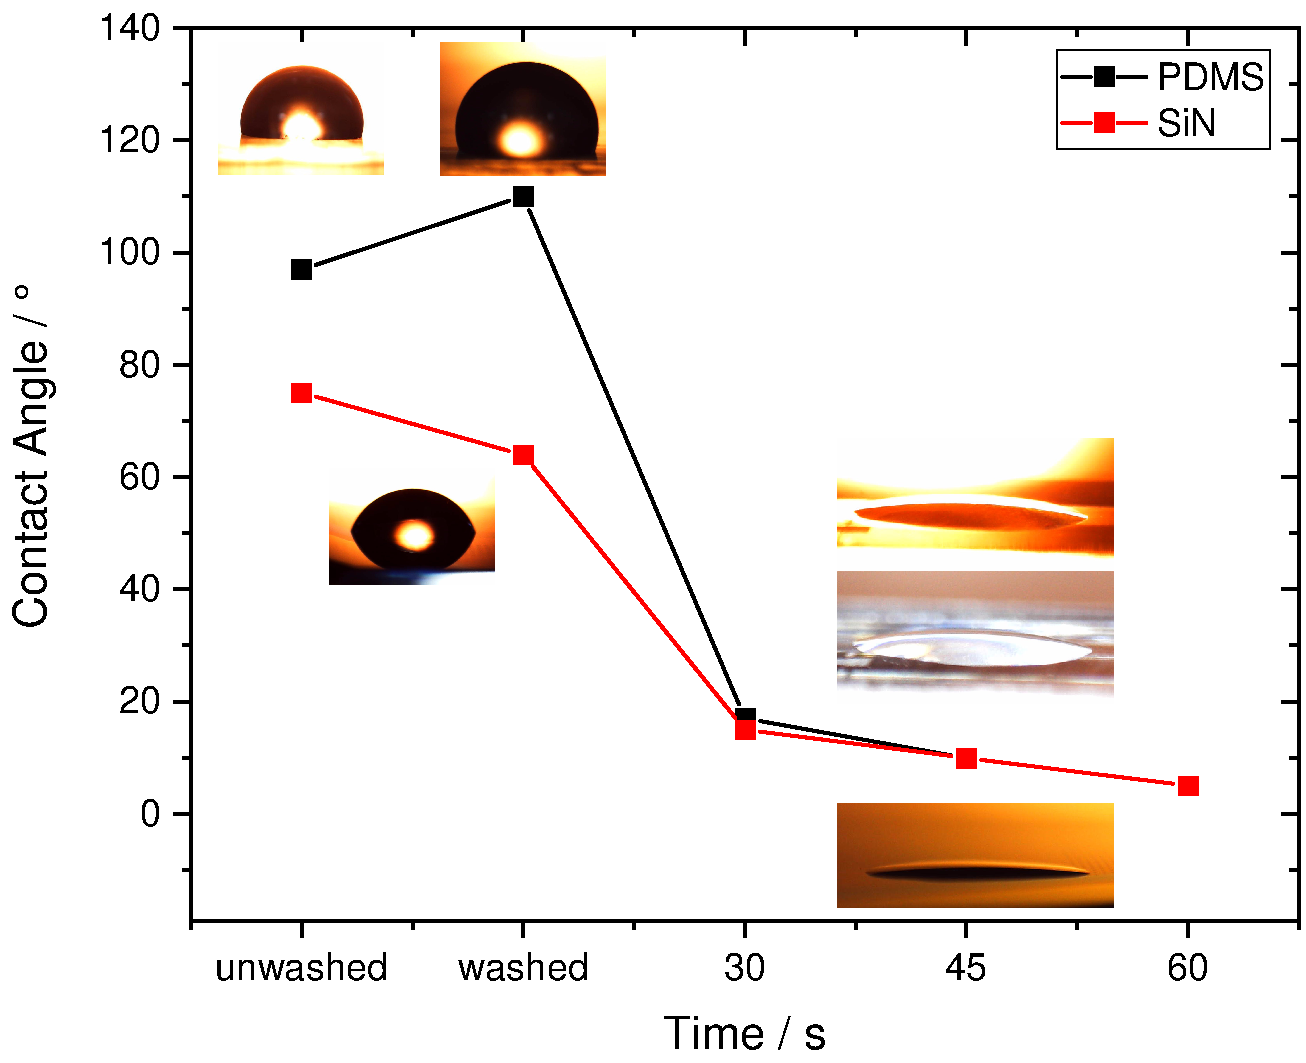
\includegraphics[height=150pt]{Ressources/ResultPlots/PDMS-sessileDrop}
	\capption{Hydrophbicity Analysis of \gls{pdms} under Plasma Exposure}{test123}
	\label{fig:coval:plasma}
\end{figure}


\subsubsection{Water-Based Approach}
Sonicate in Acetone and Water 5'
1:1 \gls{hcl}:Methanol
\gls{h2so4}
Treat for 30 min in light boiling water